%!TEX root = ../thesis.tex
%*******************************************************************************
%****************************** Fourth Chapter **********************************
%*******************************************************************************
\part{Case Studies}
\chapter{Shared Dynamics between Temporally Lagged Climate Variables: A Case Study of SST and Continental Precipitation}


% **************************** Define Graphics Path **************************
\ifpdf
    \graphicspath{{content/chapter4/figs/raster/}{content/chapter4/figs/pdf/}{content/chapter4/figs/}}
\else
    \graphicspath{{content/chapter4/figs/vector/}{content/chapter4/figs/}}
\fi

\section{Teleconnections in the Climate System}
complicated climate system, importance of teleconnections for understanding, predictions etc.; lagged teleconnections challening to analyze in a data-driven way, requires 
advanced techniques (complex rotated MCA)


\section{Climate Data}

We use ERA5 monthly averaged reanalysis \cite{c3s_era5_monthly_single} for sea surface temperature (SST) and continental precipitation to investigate the shared dynamics between these two variables on seasonal to decadal time scales. The ERA5 dataset provides global coverage on a regular longitude-latitude grid with a spatial resolution of \ang{0.25} and a monthly temporal resolution.  The time frame of the dataset spans from 1940 to today (given a couple of months delay), allowing us to capture long-term climate variability and trends and potential teleconnnections between both variables.

How is the SST data obtained in ERA5? (observations (in-situde, satellites)? model simulations? )
How is the precipitation data obtained in ERA5?

Can we trust the SST of ERA5 ?
Can we trust the prcp of ERA5 ?

By analyzing the covariability between SST and continental precipitation, we aim to identify large-scale patterns, regional impacts, and temporal relationships that can enhance our understanding of the climate system.


We focus on Geographic coverage: 40°S to 60°N with 1°x1° spatial resolution why?

We 
Data Preprocessing Steps: temporal smoothing; normalizeation, weighting, etc.



We apply theta extended, complex MCA to SST and con-
tinental precipitation using a theta period Ts 5 12 to account
for the seasonal cycle. The dimensionality of the problem can
be greatly reduced with the first 72 modes explaining more than
99\% of the lagged covariance (Fig. 4a). To simplify the ob-
tained patterns and to increase the physical meaning of the
results (section 2c), we rotate the first 150 modes explaining
99.82\% of the lagged covariance. Our decision to rotate 150 modes
is motivated by the idea of retaining as much information as
possible without including the noise that dominates the higher
modes. Since we observe a marked drop in singular values at
about the mode number 100 followed by an exponential de-
crease in singular values (Fig. 4b), we guess that there is a
negligible information content in higher modes. Moreover, the
quality of the reconstructed signal is rather independent of the
exact number of rotated modes, with 150 6 50 yielding basi-
cally identical results for the first six modes for both varimax
orthogonal and promax p 5 2 oblique rotation. Therefore, we
will restrict our discussion in the following to the first six
modes. To address the question of the rotation method to be
chosen, we note that promax oblique rotation performs better
when simple structures are present and correlations among
PCs are high (Finch 2006). We expect our first mode to be
dominated by the shared dynamics of the seasonal cycle of
both SST and continental precipitation, which is indeed what
we find for both promax (not shown here) and varimax solution
(Fig. 5). This mode, however, is fairly global and as such does
not represent a simple structure. Furthermore, we observe that
the correlations among the first six promax-rotated PCs
range from 20.15 to 0.13 only, underlining that the promax
oblique solution is close to orthogonal and differences from the varimax solutions only marginal, at least for the first six modes.
Since the promax oblique solution seemingly does not provide
a better result, we opt for the somewhat simpler varimax or-
thogonal rotation. In the following, we will discuss the varimax-
rotated modes by investigating the real part of the PCs, the
spatial amplitude and phase functions for both fields, SST and
continental precipitation, respectively.
In our representations of the modes, we remove nonsignifi-
cant, `noisy' phase values (see section 4a) by masking out
regions in the spatial amplitude and phase function exhibiting a
max-normalized amplitude of ,0.25.

\paragraph{Mode 1} Mode 1 describes 62.7\% of the covariance between SST
and continental precipitation, clearly showing the annual cycle
(Figs. 5 and 12a). As expected, the annual cycle shows itself
in both variables on a global scale, with the exception of the
equatorial ocean, where the seasonal SST variations are only
weak. The phase function correctly identifies the anticorrelation
between the northern and southern oceans. It also suggests that
the eastern equatorial Pacific and the equatorial Indian Ocean
nevertheless show a weak seasonal signal, which is, however,
positively phase shifted relative to the rest of the southern
ocean. On the continents, precipitation dominates mainly in
monsoon areas and the tropics. The phase function illustrates
the division into June–August (white) and December–February
(black) dominated rainfall systems and identifies corresponding
transition zones, as for example over the South American rain
forest and central North America. It also highlights some in-
teresting dynamical regions that stand out from their respec-
tive environments, namely, the west and east coasts of North
America, the Mediterranean region, and, to a lesser degree, the
East Asian monsoon region in China.

The obtained mode provides an instructive example to
highlight the benefits of the complexified approach due to the
mode’s corresponding narrowband frequency spectrum (Fig. 12a).
Using the dominant periodicity of mode 1, T1 5 12 months, the
interpretation of a phase shift u, given by the spatial phase
function, as time lag t is straightforward and can be computed
via t 5 T1u/(2p). Doing this for some exemplary locations
(denoted by red circles in Fig. 5), we observe that the seasonal
SST maximum of the North Pacific follows the one in the South
Pacific by 196 days, that is, being almost perfectly anti-
correlated (Fig. 6). The relative time shifts of the SST and
precipitation maximum of 81 days in the Indian Ocean and 86
days at Poyang Lake, China, is close to 3 months and as such
translates to a phase shift of about 2p/2, something that cannot
be picked up as feature within one mode when using standard
MCA. It should also be noted that although the sampling fre-
quency of SST and precipitation is monthly, the phase function
is continuous and thus allows us to infer time lags on shorter
time scales. This is, for instance, the case for the seasonal
precipitation maximum in Darwin, Australia, which precedes
the seasonal SST maximum of the South Pacific by 27 days.

\begin{figure}
    \centering
    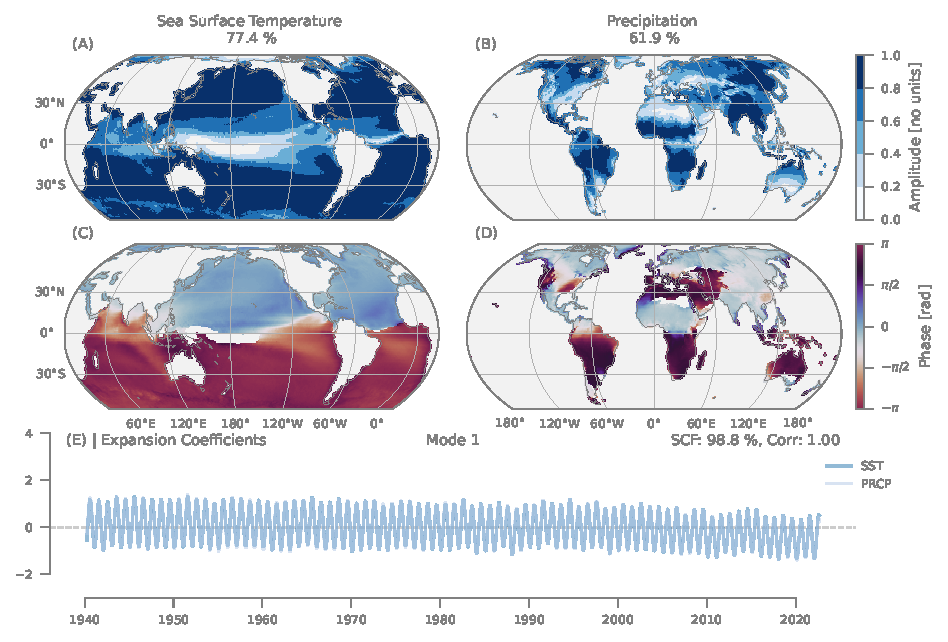
\includegraphics[width=\textwidth]{tele_mode01.pdf}
    \caption[TBD]{\textbf{Caption} Description}
    \label{fig:tele:mode01}
\end{figure}

\paragraph{Mode 2} Mode 2 (7.0\%) can be clearly associated with the ocean–
atmosphere phenomenon of ENSO (Figs. 7 and 12b). During
El Niño, higher SST in the central and eastern Pacific and lower
SST in the western Pacific positively correlate with heavier
rainfall within a narrow band along the west coast and the
southeastern coast of South America (Tedeschi et al. 2013), the
east and west coasts of North America (Ropelewski and
Halpert 1986), the East Asian monsoon region (Wen et al.
2019), and the Horn of Africa (Indeje et al. 2000). At the same
time, precipitation decreases in northern South America
(Tedeschi et al. 2013), Oceania (Dai and Wigley 2000), South
Africa (Gaughan et al. 2016), and the Indian monsoon region
(Cherchi and Navarra 2013). During La Niña (the counter-
phase of El Niño), these correlations are reversed. Recently,
similar teleconnections have been identified via event coinci-
dence analysis (Wiedermann et al. 2021). For a current sum-
mary of established ENSO-related rainfall patterns during El
Niño and La Niña see Lenssen et al. (2020).

Our result also shows the dynamical link between ENSO in
the Pacific Ocean and the Indian Ocean (Krishnamurthy and
Kirtman 2003), the South China Sea (Klein et al. 1999), and the
tropical North Atlantic (Enfield and Mayer 1997; Saravanan
and Chang 2000; Alexander and Scott 2002; Chiang and Sobel
2002) in accordance with previous studies. Interestingly, it was
found that the ENSO-related SST teleconnections in the re-
mote oceans often occur with some delays, with the Indian
Ocean typically peaking ;3 months and the South China Sea
and tropical North Atlantic ;5 months after the SST peak in
the Pacific ENSO region (Enfield and Mayer 1997; Klein et al.
1999; Saravanan and Chang 2000). The mechanism behind
these lagged responses, known as the atmospheric bridge, is
based on the characteristic atmospheric circulation during El
Niño, which causes changes in cloud cover and evaporation
over the remote oceans, leading to increased net heat flux and
SSTs (Lau and Nath 1996; Klein et al. 1999). However, due to
the broadband frequency spectrum of the SST PC (Fig. 12b),
with most of the energy contained at four different peaks
around 2.5, 3.5, 5, and 11 years, the phase cannot simply be
translated into a time shift. Nevertheless, the tropical North
Atlantic clearly exhibits more positive phase values compared
to the Pacific El Niño region, therefore indicating to be posi-
tively time shifted relative to the Pacific.

\begin{figure}
    \centering
    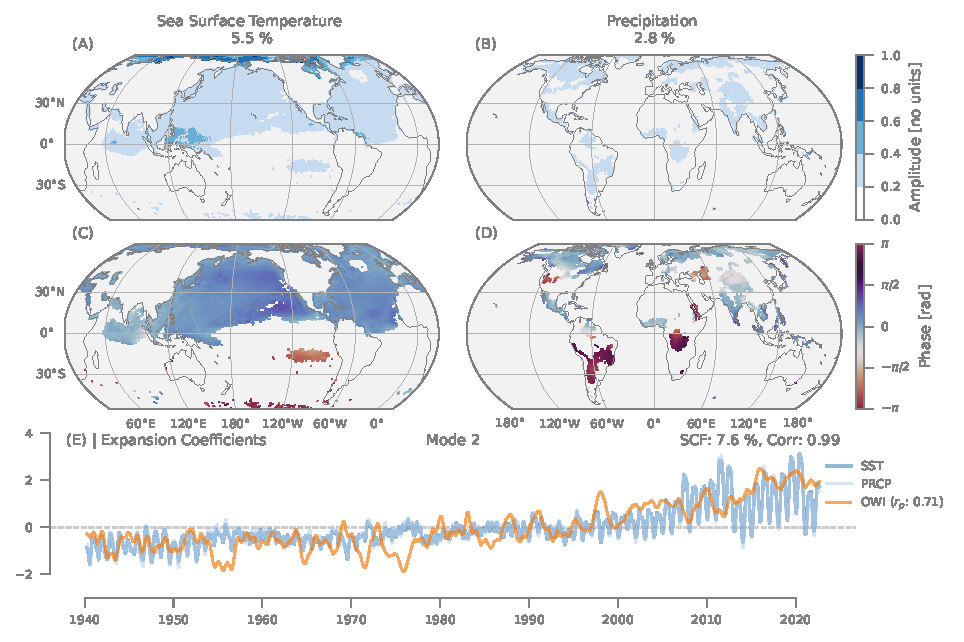
\includegraphics[width=\textwidth]{tele_mode02.pdf}
    \caption[TBD]{\textbf{Caption} Description}
    \label{fig:tele:mode02}
\end{figure}


\paragraph{Mode 3} Mode 3 (6.9\%) represents global warming and the associ-
ated changes in precipitation patterns (Fig. 8). The warming
SST patterns clearly emerge in all major ocean basins, although
more pronounced in the Northern Hemisphere due to the
asymmetric response of the northern and southern trade winds
to global warming (Xie et al. 2010). We also note a pronounced
warming of the western part of both the Pacific and the
Atlantic basins, both regions of enhanced ocean heat transport
(Xie et al. 2010; Hannachi and Trendafilov 2017). Similar to
these oceanic trends, we also observe global trends in the precipi-
tation patterns, with decreasing rainfall over the Mediterranean,
South Africa, Australia, South America, and parts of western
North America. There seems to be also a decrease of rainfall
over the west Asian monsoon region. In contrast to that, the
results suggest increased precipitation over the Indian mon-
soon region as well as some localized regions in Europe and in
South and North America. These results are largely in agreement
with studies based on observational data (Gu and Adler 2015)
and, more recently, on CMIP5 climate simulations (Giorgi
et al. 2019). Finally, it should be stressed that both PCs, SST
and precipitation, only provide a meaningful interpretation for
phases u ’ 0; 6p (correlation, anticorrelation), due to their
broadband frequency spectra (Fig. 12c). For phase shifts dif-
ferent from that, no clear conclusions can be drawn, as for
example is the case for equatorial Africa where the phase shift
is approximately 1p/2.


\begin{figure}
    \centering
    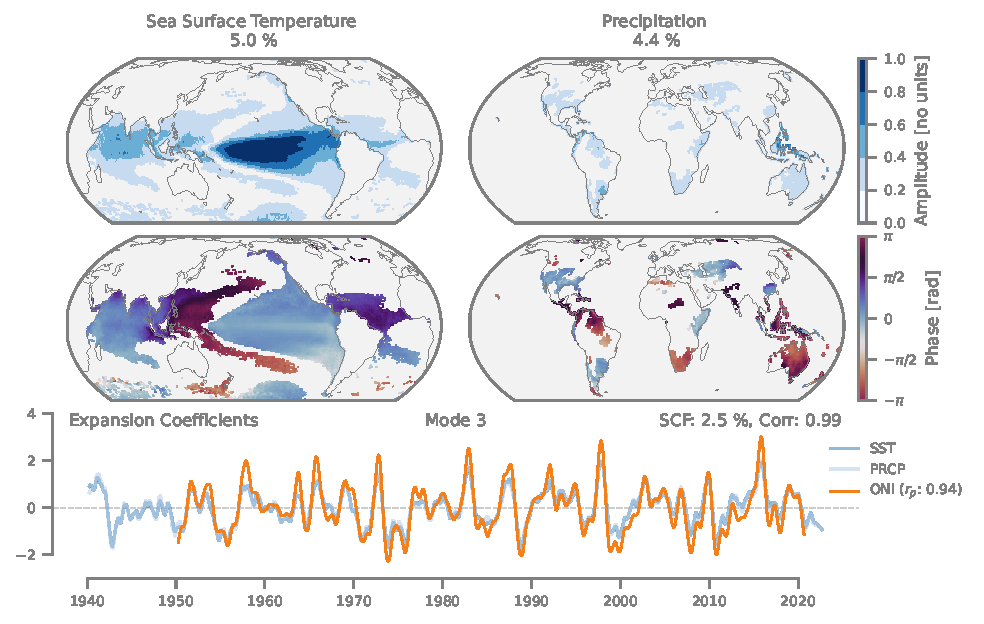
\includegraphics[width=\textwidth]{tele_mode03.pdf}
    \caption[TBD]{\textbf{Caption} Description}
    \label{fig:tele:mode03}
\end{figure}


\paragraph{Mode 4} Mode 4 (1.6\%) shows a slow-oscillating pattern of SST in
the northeastern Pacific correlating with localized precipitation
patterns distributed over all continents (Fig. 9). The typical
spatial SST pattern is known as the Pacific decadal oscillation
(PDO) (Mantua et al. 1997) and a well-established climate
index. A combination of various processes originating in the
tropics and extratropics has been proposed as the physical
source of the PDO (Newman et al. 2016), with ENSO and PDO
likely responding to the same forcing function (Pierce 2002).
Our analysis, however, provides a means to disentangle ENSO-
and PDO-related precipitation patterns, which are often similar
for western North America (Hu and Huang 2009), although
it also reveals important differences (e.g., for Australia, the
Indian subcontinent, or the African Sahel region). Yet care must
be taken when interpreting regions that have a phase shift
different from 0, 6p. Although the PDO exhibits a strong
spectral energy at about 35 years, the mode contains also im-
portant features at about 1–4 years (Fig. 12d), making the
phase interpretation physically less clear.


\begin{figure}
    \centering
    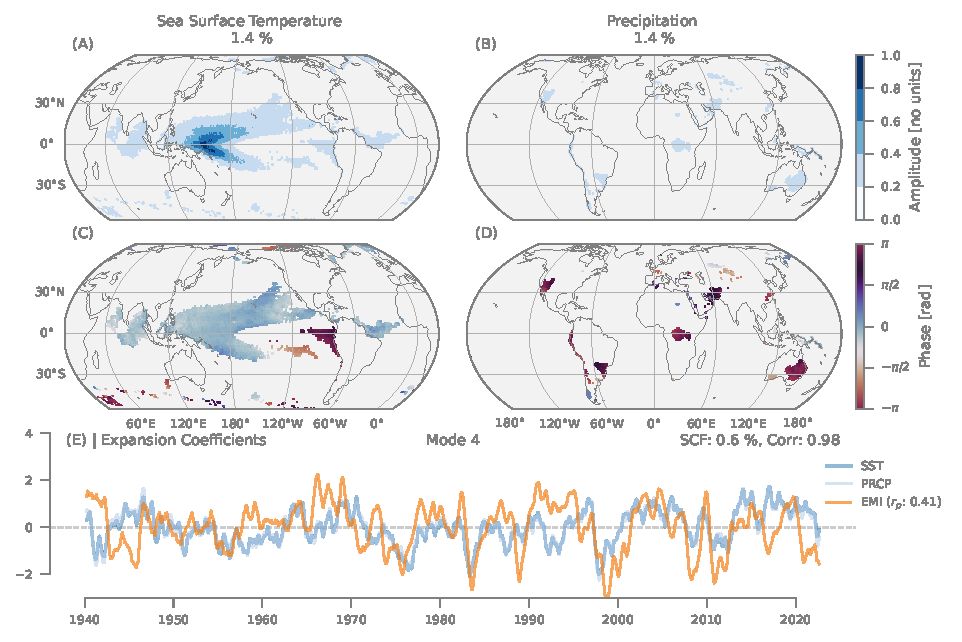
\includegraphics[width=\textwidth]{tele_mode04.pdf}
    \caption[TBD]{\textbf{Caption} Description}
    \label{fig:tele:mode04}
\end{figure}


\paragraph{Mode 5} Mode 5 (1.6\%) describes an oscillating SST anomaly mainly
limited to the central Pacific (Figs. 10 and 12e) describing
El Niño Modoki (Ashok et al. 2007) and represented by the
EMI. Higher SST in the central Pacific and lower SST in the
eastern Pacific correlate with reduced precipitation in the East
Asian monsoon region (Feng et al. 2011), Australia (Taschetto
and England 2009), parts of South America (Tedeschi et al.
2013), and South Africa (Ratnam et al. 2014) and vice versa.
Some of these teleconnections have recently been revealed by
event coincidence analysis (Wiedermann et al. 2021) although
important links to the East Asian monsoon region, for example,
were missing. Although our result suggests that continental
rainfall in certain regions of Africa, Arabia, and the Americas
are phase-shifted El Niño Modoki expressions, future work has
to show if these weak amplitudes are significant.

\begin{figure}
    \centering
    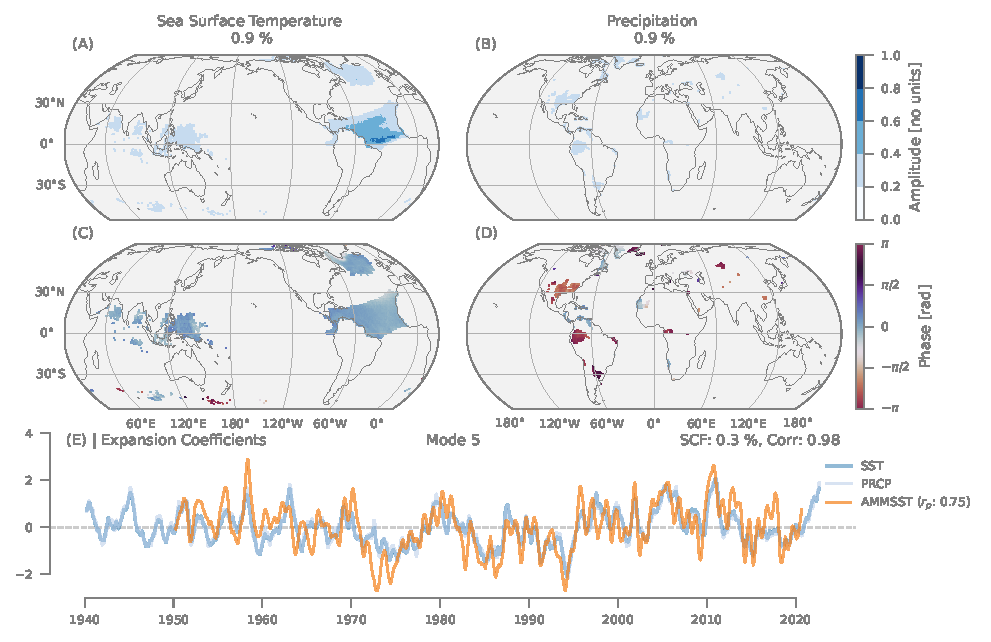
\includegraphics[width=\textwidth]{tele_mode05.pdf}
    \caption[TBD]{\textbf{Caption} Description}
    \label{fig:tele:mode05}
\end{figure}


\paragraph{Mode 6} Mode 6 (1.1\%) is characterized by an SST pattern con-
centrated in the tropical and subarctic North Atlantic (Figs. 11
and 12f). The SST pattern, representing the Atlantic meridio-
nal mode (AMM), is the dominant coupled ocean–atmospheric
phenomenon in the tropical Atlantic (Servain et al. 1999) and
its impacts on precipitation of the African Sahel zone, Central
America, and northern South American continent are well
known (Lamb et al. 1986; Martin et al. 2014). Only very re-
cently, Vittal et al. (2020) found a link between the AMM and
Indian summer monsoon rainfall, which they used to improve
precipitation forecast. In addition, our result suggests more
teleconnections between the AMM and precipitation vari-
ability over the Mediterranean, East Africa, the Congo basin,
North America, and the East Asian monsoon region, pro-
viding much potential for advancing local rainfall predic-
tions in those areas. Due to the missing intrinsic time scale
with no clear periodicity (Fig. 12f), only correlating and anti-
correlating patterns should be interpreted. However, most of
the regions identified by this mode satisfy being correlated or
anticorrelated.



\begin{figure}
    \centering
    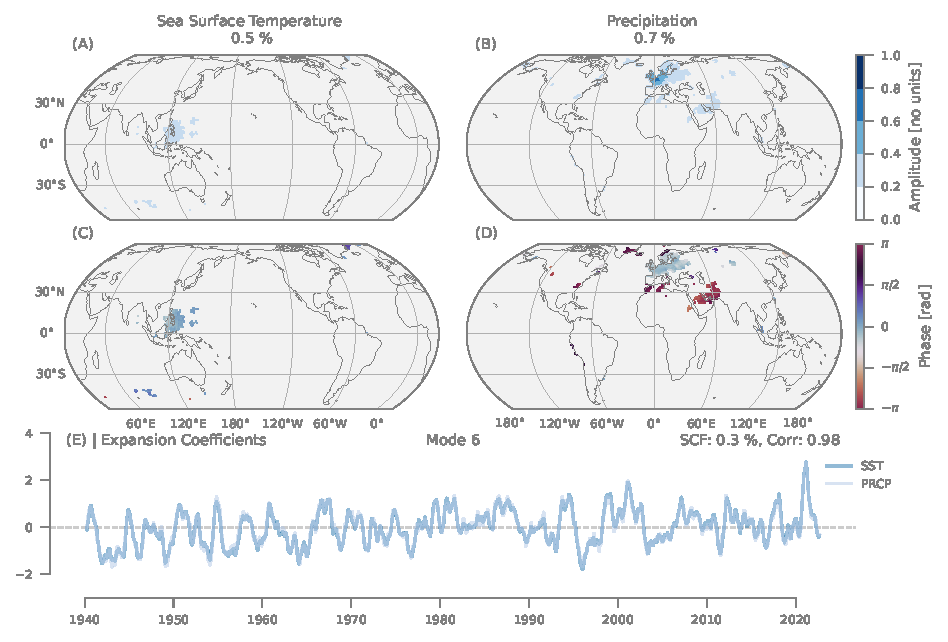
\includegraphics[width=\textwidth]{tele_mode06.pdf}
    \caption[TBD]{\textbf{Caption} Description}
    \label{fig:tele:mode06}
\end{figure}

\begin{figure}
    \centering
    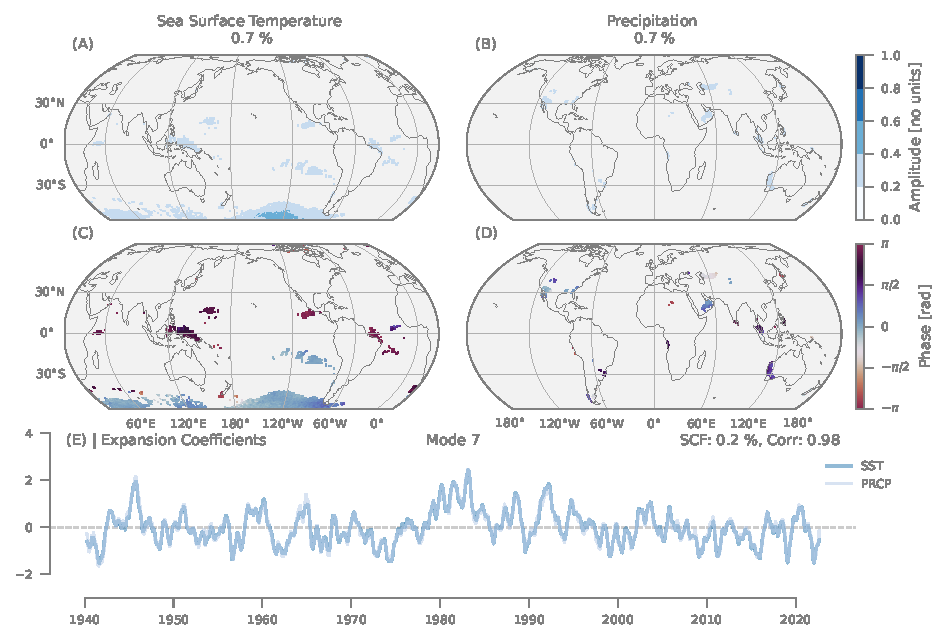
\includegraphics[width=\textwidth]{tele_mode07.pdf}
    \caption[TBD]{\textbf{Caption} Description}
    \label{fig:tele:mode07}
\end{figure}

\begin{figure}
    \centering
    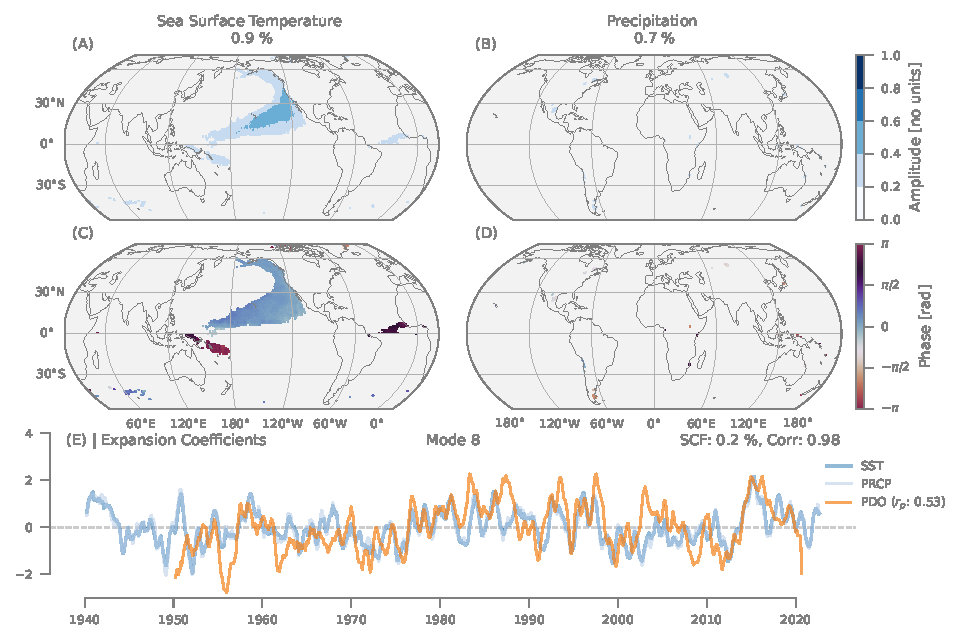
\includegraphics[width=\textwidth]{tele_mode08.pdf}
    \caption[TBD]{\textbf{Caption} Description}
    \label{fig:tele:mode08}
\end{figure}

\section{Results}
Identification of large scale patterns: Seasonal Cycle; El Niño-Southern Oscillation (ENSO), Detection of ENSO-related patterns, spatial distribution of 
SST anomalies and their correlation with precipitation changes; Implications for predicting ENSO impacts on global weather patterns;
Global Warming Trend; Identification of trends in SST and precipitation linked to global warming; Regional analysis of warming effects and 
their correlation with precipitation changes; Pacific Decadal Oscillation (PDO); analysis of PDO patterns and their influence on climate variability;
Temporal lag and phase relationships between SST and precipitation during PDO events; ENSO Modoki; Detection of ENSO Modoki patterns; Differences from 
canonical ENSO and their specific impacts on regional climates; Atlantic Meridional Mode (AMM); Identification of AMM-related variability; Correlation between 
SST in the Atlantic and precipitation in adjacent continental regions; 

Key Findings and Insights:
Enhanced Understanding of Teleconnections; Insights into long-distance correlations between ocean and atmospheric variables; Identification of key regions and time lags 
in climate interactions; Improved Predictive Capabilities; Contributions to more accurate climate models by incorporating lagged relationships; Potential applications 
in seasonal and long-term climate forecasting; 

Regional Climate Insights
Detailed analysis of regional climate phenomena and their broader implications
Identification of regions with strong seasonal and interannual variability

Conclusion
Summary of key findings from the application of complex rotated MCA on climate variables
Implications for future climate research and potential areas for further study
Final thoughts on the importance of advanced data analysis techniques in enhancing our understanding of climate systems




\section{Power Spectral Density}
\mynote{check out \url{https://kls2177.github.io/Climate-and-Geophysical-Data-Analysis/chapters/Week6/filtering_in_freq3.html}}


\begin{figure}
    \centering
    
\includegraphics[width=\textwidth]{tele_psd.pdf}
    \caption[TBD]{\textbf{Caption} Description}
    \label{fig:tele:psd}
\end{figure}


\section{Case Study 2: Representation of the Madden-Julian Osciallation}
sub-seasonal time scales 
